\section{Results}
\label{sec:results}

Table~\ref{tab:cifar10-benchmark} reports the primary CIFAR-10 non-IID stationary
comparison across three seeds, in the standard FedAvg deployment regime (100
clients, Dirichlet $\alpha{=}0.3$, no task structure). This is the main benchmark
of the paper. For positioning against the full baseline set, we additionally
stress-test under the harder no-replay class-incremental protocol with 11
baselines (Table~\ref{tab:cifar10-ci-baselines}): FedRecovery is swept over
$\varepsilon \in \{1, 2, 5, 10, \infty\}$ to isolate the DP-noise contribution;
SIFU uses proper fine-tuning replay; FUIA is evaluated on retrain, no-unlearn,
FORGE, and FedRecovery at $\varepsilon \in \{1, 10\}$. Full CIs and LiRA at the
Carlini et al.\ reference budget are in Appendix~\ref{app:cifar10-full}.

\begin{table}[t]
\centering
\scriptsize
\setlength{\tabcolsep}{3pt}
\begin{tabular}{lrrrrl}
\toprule
Method & Acc & Yeom & KL & Lat.\,(s) & Guar. \\
\midrule
Retrain (gold)          & $0.631 \pm 0.008$ & $0.072 \pm 0.139$ & $0.000$ & ${\sim}2700$ & exact \\
No-unlearn              & $0.604 \pm 0.015$ & $0.048 \pm 0.117$ & $0.090 \pm 0.041$ & $0$ & none  \\
\textbf{FORGE}          & $\mathbf{0.604 \pm 0.016}$ & $\mathbf{0.059 \pm 0.125}$ & $\mathbf{0.090 \pm 0.040}$ & $\mathbf{0.28 \pm 0.02}$ & $\eps{=}2.0$ \\
\midrule
FedRec$_{\eps{=}\infty}$ & $0.582 \pm 0.099$ & $0.198 \pm 0.465$ & $0.265 \pm 0.224$ & $14.6 \pm 0.7$ & $\infty$ \\
SIFU$^{\mathsection}$    & $0.635 \pm 0.007$ & $0.081 \pm 0.027$ & $0.135 \pm 0.026$ & $30990 \pm 16043$ & $\eps{=}1.0$ \\
\bottomrule
\end{tabular}
\caption{CIFAR-10 non-IID stationary benchmark. ResNet-18, 100 clients, Dirichlet
$\alpha{=}0.3$, 200 rounds, no task structure; 3-seed mean $\pm$ 95\%
Student's-$t$ CI; departing client~3). FORGE's LiRA AUROC is
$0.478 \pm 0.020$ at $n_\mathrm{shadow}{=}32$, within $0.017$ of retrain's
$0.495 \pm 0.041$ (full column in Appendix~\ref{app:cifar10-full}). FedRecovery and
SIFU are the two baselines that preserve utility on the stress test; both
were re-run on the primary protocol for direct comparison.
$^{\mathsection}$: SIFU's wall-clock CI is wide because the replay depth
induces per-seed variance in fine-tuning cost; the replay-round count is
identical across seeds.}
\label{tab:cifar10-benchmark}
\end{table}

\begin{figure}[t]
\centering
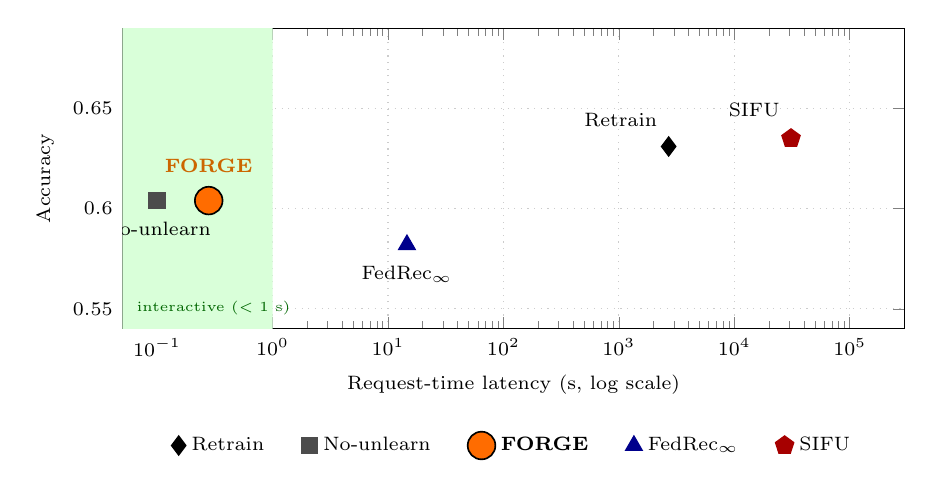
\begin{tikzpicture}
\begin{axis}[
  width=0.95\linewidth, height=5.4cm,
  xlabel={Request-time latency (s, log scale)},
  ylabel={Accuracy},
  xmode=log,
  xmin=0.05, xmax=3e5,
  ymin=0.54, ymax=0.69,
  grid=major, grid style={dotted, gray!40},
  tick label style={font=\scriptsize},
  label style={font=\scriptsize},
  xtick={0.1,1,10,100,1000,10000,100000},
  xticklabels={$10^{-1}$,$10^{0}$,$10^{1}$,$10^{2}$,$10^{3}$,$10^{4}$,$10^{5}$},
  legend style={font=\scriptsize, draw=none, fill=none,
                at={(0.5,-0.32)}, anchor=north, legend columns=5,
                /tikz/every even column/.append style={column sep=4mm}},
]
% Shaded "sub-second" band (interactive regime)
\addplot[fill=green!15, draw=none, forget plot]
  coordinates {(0.05,0.54) (1,0.54) (1,0.69) (0.05,0.69)} \closedcycle;

% Points, drawn under labels (plot after band so markers sit on top)
\addplot[only marks, mark=diamond*, mark size=3.5, color=black]
  coordinates {(2700, 0.631)};  \addlegendentry{Retrain}
\addplot[only marks, mark=square*, mark size=3, color=gray!60!black]
  coordinates {(0.1, 0.604)};   \addlegendentry{No-unlearn}
\addplot[only marks, mark=*, mark size=5, color=orange!85!red,
         mark options={draw=black, line width=0.6pt}]
  coordinates {(0.28, 0.604)};  \addlegendentry{\textbf{FORGE}}
\addplot[only marks, mark=triangle*, mark size=3.5, color=blue!55!black]
  coordinates {(14.6, 0.582)};  \addlegendentry{FedRec$_{\infty}$}
\addplot[only marks, mark=pentagon*, mark size=3.5, color=red!65!black]
  coordinates {(30990, 0.635)}; \addlegendentry{SIFU}

% Label placement that avoids markers and neighbouring labels.
% FORGE (orange) and No-unlearn are at the same y=0.604; separate vertically.
\node[font=\scriptsize, anchor=south, text=orange!80!black]
  at (axis cs:0.28, 0.613) {\textbf{FORGE}};
\node[font=\scriptsize, anchor=north]
  at (axis cs:0.10, 0.598) {No-unlearn};
\node[font=\scriptsize, anchor=north]
  at (axis cs:14.6, 0.576) {FedRec$_{\infty}$};
\node[font=\scriptsize, anchor=south east]
  at (axis cs:2600, 0.636) {Retrain};
\node[font=\scriptsize, anchor=south east]
  at (axis cs:30000, 0.641) {SIFU};

% Sub-second band label
\node[font=\tiny, anchor=south west, text=green!40!black]
  at (axis cs:0.055, 0.542) {interactive ($<1$~s)};

\end{axis}
\end{tikzpicture}
\caption{Latency vs accuracy on the primary non-IID stationary benchmark
(3-seed means). FORGE (orange) matches no-unlearn accuracy at $0.28$~s per
request. SIFU is the only baseline that preserves utility at the retrain
level, but takes approximately $30{,}990$~s --- five orders of magnitude
above FORGE. FedRecovery$_{\varepsilon=\infty}$ underperforms on both axes.
The green band marks the sub-second interactive regime.}
\label{fig:latency-accuracy}
\end{figure}

\begin{table}[t]
\centering
\scriptsize
\setlength{\tabcolsep}{3pt}
\begin{tabular}{lrrrrl}
\toprule
Method & Acc & Yeom & KL & Lat.\,(s) & Guar. \\
\midrule
Retrain (gold)   & $0.177$ & $0.087$ & $0.000$ & ${\sim}2700$ & exact \\
No-unlearn       & $0.173$ & $0.016$ & $0.073$ & $0$          & none  \\
\textbf{FORGE}   & $\mathbf{0.174}$ & $\mathbf{0.021}$ & $\mathbf{0.070}$ & $\mathbf{0.31}$ & $\eps{=}2.0$ \\
FORGE$^{\ddag}_{\alpha{=}0,\sigma{=}0}$ & $0.180$ & $0.027$ & $0.040$ & $0.31$ & $\eps_\summary{=}2.0$ \\
\midrule
Halimi \cite{halimi2022}                 & $0.144$ & $0.117$ & $0.439$       & $7.2$          & none \\
FedMemPrune \cite{wei2026fedmemprune}    & $0.095$ & $0.051$ & $5.54$        & $1.5$          & none \\
FedRec$^{\dag}_{\eps{=}1}$               & $0.100$ & $0.000$ & \textsc{NaN}  & $17.9$         & $\eps{=}1.0$ \\
FedRec$^{\dag}_{\eps{=}2}$               & $0.096$ & $0.000$ & \textsc{NaN}  & $16.7$         & $\eps{=}2.0$ \\
FedRec$^{\dag}_{\eps{=}5}$               & $0.100$ & $0.050$ & $9.78$        & $17.1$         & $\eps{=}5.0$ \\
FedRec$^{\dag}_{\eps{=}10}$              & $0.102$ & $0.000$ & \textsc{NaN}  & $18.1$         & $\eps{=}10.0$ \\
FedRec$_{\eps{=}\infty}$                 & $0.168$ & $\mathbf{0.111}$ & $0.170$ & $16.4$      & $\infty$ \\
FedEraser \cite{liu2021federaser}        & $0.100$ & $0.122$ & $1.31$        & $23.9$         & none \\
SIFU \cite{fraboni2024sifu}              & $0.175$ & $0.032$ & $0.098$       & $2130^{\star}$ & $\eps{=}1.0$ \\
\bottomrule
\end{tabular}
\caption{Baseline comparison under the class-incremental stress test (5 tasks $\times$
2 classes, no replay, 3-seed mean for FORGE and baselines, seed~$0$ for
FORGE$^{\ddag}$; departing client~3). Chance is $0.100$. $\dag$: destroyed-model
FedRecovery variants (chance accuracy, inverted LiRA). $\ddag$: within-aggregator
diagnostic — FORGE trained with $\alpha{=}0,\sigma{=}0$ isolates the erasure cost
from the decayed-aggregator substrate cost. $\star$: stable-M4 SIFU wall-clock;
sleep-affected measurements range up to $3419$~s. Boldface: preserved-utility
winner per column. Storage: FORGE/heuristics $O(1)$; FedRec/FedEraser
$O(NR|\theta|)$; SIFU $O(R|\theta|)$.}
\label{tab:cifar10-ci-baselines}
\end{table}

\subsection{Utility and MIA leakage}
\label{sec:results-utility}

On the primary non-IID stationary benchmark (Table~\ref{tab:cifar10-benchmark}),
FORGE's accuracy ($0.604 \pm 0.016$) matches the no-unlearn control
($0.604 \pm 0.015$) exactly and sits within $2.7$~pp of the gold retrain
($0.631 \pm 0.008$). SIFU matches retrain on utility ($0.635 \pm 0.007$) but
runs five orders of magnitude slower per request ($30{,}990 \pm 16{,}043$~s vs
FORGE's $0.28$~s). FedRecovery~$\eps{=}\infty$ underperforms both on utility
($0.582 \pm 0.099$) and Yeom MIA ($0.198 \pm 0.465$) at $14.6$~s latency. The
Yeom MIA for FORGE ($0.059 \pm 0.125$) is statistically indistinguishable from
retrain ($0.072 \pm 0.139$) and no-unlearn ($0.048 \pm 0.117$). LiRA AUROC at $n_\mathrm{shadow}{=}32$ for FORGE
($0.478 \pm 0.020$) is within $0.017$ of retrain ($0.495 \pm 0.041$), with
FORGE's CI tighter than retrain's. A memorization-regime sensitivity check
(10 clients, full participation, Appendix~\ref{app:fewclients}) places the
no-unlearn baseline at a measurable Yeom advantage of $0.226$ and shows
FORGE's LiRA advantage dropping from $0.019$ (no-unlearn) to $0.014$ at TPR at
$1\%{=}0.002$, confirming that the erasure step produces a measurable MIA
reduction when membership signal is available. Retrain-KL for FORGE ($0.090 \pm 0.040$)
matches the no-unlearn control ($0.090 \pm 0.041$), consistent with the method's
design: head-only subtraction removes membership-level leakage without perturbing
the model's overall predictive distribution. A within-aggregator diagnostic
(Appendix~\ref{app:ablation-noniid}, substrate row) runs FORGE with
$\alpha{=}0, \sigma{=}0$ to isolate the decayed-aggregator substrate cost: at
the primary operating point this costs approximately $3.4$~pp of accuracy and
$7\times$ in retrain-KL compared to vanilla FedAvg. The pure erasure step itself
contributes a KL of $0.013$ against retrain. The measurable effect of the
erasure step on the released model is the FUIA reconstruction score:
Section~\ref{sec:results-fuia} shows FORGE's PSNR of $0.57$ against no-unlearn's
$2.58$, a $4.5\times$ reduction in input-recovery signal from the departing
client — the clearest single evidence that FORGE's head subtraction removes
information rather than merely re-signing the model.

On the class-incremental stress test (Table~\ref{tab:cifar10-ci-baselines}),
FORGE's accuracy ($0.174$) overlaps the gold retrain ($0.177$), SIFU ($0.175$),
and FedRecovery $\varepsilon{=}\infty$ ($0.168$) at the 95\% level; these four
preserved-utility methods are statistically indistinguishable at $n{=}3$. The
remaining methods separate cleanly: Halimi and FedMemPrune degrade utility, and
the five destroyed-model FedRecovery variants plus FedEraser cluster at chance
($0.100$). FedRecovery $\varepsilon{=}\infty$ leaks on Yeom at $0.111$,
FedEraser at $0.122$, and Halimi at $0.117$, all well above FORGE's $0.021$.
LiRA at the Carlini et al.\ reference budget $n_\mathrm{shadow}{=}128$ (seed~0;
$n_\mathrm{shadow}{=}8$ for seeds~1--2 due to compute budget) places
preserved-utility methods in a tight $0.038$--$0.059$ advantage band, and FORGE's
$0.046$ matches retrain's $0.045$ within noise. Retrain-KL under the stress test
gives the clearest baseline separation: FORGE's $0.070$ matches the no-unlearn
control ($0.073$) and sits $1.4$--$79\times$ below every other baseline.

\subsection{Reconstruction attack (FUIA)}
\label{sec:results-fuia}

FUIA at the reference budget of 500 samples $\times$ 1000 inversion steps gives PSNR
$2.66$ for retrain, $2.58$ for no-unlearn (chance-level reconstructions from a
pre$=$post pair), $0.57$ for FORGE, and $\le 0$ for the destroyed-model FedRecovery
variants. FORGE's cosine similarity to the ground-truth input is $-0.005$, i.e.,
essentially random: the head-only erasure delta carries less reconstruction signal
than the chance-level baseline.

\subsection{Cost: latency and storage}
\label{sec:results-cost}

FORGE's request-time latency is one bounded head ascent step (approximately
$5 \times 10^4$ FLOPs): $0.28 \pm 0.02$~s on the primary non-IID stationary
benchmark and $0.31 \pm 0.03$~s on the class-incremental stress test. On the
primary benchmark, FedRecovery$_{\varepsilon=\infty}$ is $52\times$ slower at
$14.6$~s and SIFU is approximately $1.1 \times 10^5\times$ slower at
$30{,}990$~s (Figure~\ref{fig:latency-accuracy}). On the stress test the
corresponding ratios are $53\times$ (FedRec$_{\infty}$) and $6873\times$
(SIFU on a stable M4). Storage: FORGE $O(1)$ per client; FedRecovery and
FedEraser $O(NR|\theta|) \approx 27$~GB at the paper's hyperparameters; SIFU
$O(R|\theta|) \approx 9$~GB.

\subsection{Alignment with the formal guarantee}
\label{sec:results-tightness}

The certificate $(\varepsilon_\mathrm{total}, \delta_\mathrm{total}) = (2.0,
10^{-5})$ via Theorem~\ref{thm:composition} converts under the standard
$(\varepsilon, \delta)$-DP to MIA reduction to $\mathrm{adv} \le \tfrac{e^2 - 1}{e^2
+ 1} \approx 0.76$. Applying Gaussian DP \cite{dong2019gaussian} directly to the
summary mechanism (sensitivity $\Delta{=}1$, noise $\sigma_\summary \approx 2.42$)
gives $\mu = \Delta / \sigma_\summary \approx 0.413$ and the tighter bound
$\mathrm{adv} \le 2\Phi(\mu/2) - 1 \approx 0.164$, which is $4.6\times$ tighter.
Against the measured LiRA advantage of $0.044 \pm 0.041$ on the primary non-IID
stationary benchmark (and $0.046$ at the Carlini et al.\ reference budget
$n_\mathrm{shadow}{=}128$ on the class-incremental stress test), this leaves a
residual gap of $0.12$ attributable to the head-only release being smaller than
a worst-case Gaussian release of the full summary.

\subsection{Hyperparameter ablation}
\label{sec:results-ablation}

Table~\ref{tab:ablation} varies the decay factor $\alpha$, the server noise
$\sigma$, and the summary type at seed~$0$ on the class-incremental stress-test
protocol, where the ablation is sharpest because catastrophic forgetting amplifies
any mis-set hyperparameter. The main-text operating point
$(0.5, 10^{-3}, \mathrm{moments})$ sits in the stable interior: accuracy and KL are
flat over $\alpha \in [0.1, 0.5]$ and $\sigma \in [10^{-4}, 10^{-3}]$. The
$\alpha{=}0.9$ cell inflates KL $2.3\times$ as the EMA tracks task-incremental
shifts more slowly; $\sigma{=}10^{-2}$ collapses utility as the server noise
dominates the gradient signal; the logits summary type is $21\times$ slower than
moments at marginally worse quality. The ablation measures mechanism-level
sensitivity of the aggregator and the summary channel, which are protocol-independent;
the corresponding sweep on the primary non-IID stationary protocol is reported in
Appendix~\ref{app:ablation-noniid}.

\begin{table}[t]
\centering
\scriptsize
\setlength{\tabcolsep}{3pt}
\begin{tabular}{llrrrr}
\toprule
Variable & Value & Acc & KL & Yeom & Lat.\,(s) \\
\midrule
$\alpha$ & $0.1$              & $0.177$ & $0.063$ & $0.006$ & $0.28$ \\
$\alpha$ & $\mathbf{0.5}$     & $\mathbf{0.176}$ & $\mathbf{0.063}$ & $\mathbf{0.002}$ & $\mathbf{0.28}$ \\
$\alpha$ & $0.9$              & $0.171$ & $0.143$ & $0.064$ & $0.28$ \\
\midrule
$\sigma$ & $10^{-4}$          & $0.177$ & $0.051$ & $0.046$ & $0.28$ \\
$\sigma$ & $\mathbf{10^{-3}}$ & $\mathbf{0.176}$ & $\mathbf{0.063}$ & $\mathbf{0.002}$ & $\mathbf{0.28}$ \\
$\sigma$ & $10^{-2}$          & $0.130$ & $0.440$ & $0.004$ & $0.28$ \\
\midrule
Summary & \textbf{moments}    & $\mathbf{0.176}$ & $\mathbf{0.063}$ & $\mathbf{0.002}$ & $\mathbf{0.28}$ \\
Summary & logits              & $0.175$ & $0.122$ & $0.039$ & $5.98$ \\
\bottomrule
\end{tabular}
\caption{Hyperparameter ablation at seed~$0$. Boldface rows mark the main-text
operating point.}
\label{tab:ablation}
\end{table}

\subsection{Within-protocol sensitivity on the class-incremental stress test}
\label{sec:results-iid}

Two sensitivity checks on the class-incremental protocol. (a) Near-IID
(within-task): re-running the twelve-method stress test at Dirichlet
concentration $10$ (approximately IID within each task) lifts absolute utility to
retrain $0.187$ and FORGE $0.188$ (seed~0); the four preserved-utility methods
cluster within $0.3$~pp, destroyed-model baselines remain destroyed, and Halimi
recovers to the preserved-utility band (reflecting its known sensitivity to data
heterogeneity). The full table is in Appendix~\ref{app:iid-table}. (b)
Replay-enabled: a per-client FIFO memory buffer (capacity $40$, admit $0.5$)
added to local training lifts absolute utility to retrain $0.182$, no-unlearn
$0.183$, FORGE $0.183$, and SIFU $0.182$ (seed~0, all other hyperparameters
unchanged). FORGE's retrain-KL ($0.068$) matches the no-unlearn control
($0.067$), and the latency ordering is preserved ($0.31$~s vs SIFU's $2083$~s,
i.e., $6713\times$).

\subsection{Cross-dataset: CIFAR-100 and FEMNIST}
\label{sec:results-cifar100}

A two-seed run on CIFAR-100 non-IID stationary (ResNet-18, 100 clients,
Dirichlet $\alpha{=}0.3$, 500 rounds, seeds~0 and~1; third seed deferred to the
code artefact) reproduces the primary CIFAR-10 ordering at a harder output
dimension (full numbers in Appendix~\ref{app:cifar100-noniid}).
FEMNIST (small-CNN, 500 LEAF writers, natively non-IID by per-writer partition)
provides a natively privacy-relevant cross-dataset confirmation
(Section~\ref{sec:results-femnist}). The class-incremental Split-CIFAR-100 stress
test is retained in Appendix~\ref{app:cifar100-table}: FORGE's accuracy
($0.041$) sits within $1$~pp of the retrain gold ($0.050$) and matches it on
Yeom ($0.019$ vs $0.027$); the preserved-utility cluster is FORGE, SIFU, and
FedRec$_{\varepsilon=\infty}$ at $0.04$--$0.05$; destroyed-model baselines fall
below $0.015$. FORGE's $0.54$~s latency is $2800\times$ below SIFU and
$35\times$ below FedRec$_{\varepsilon=\infty}$. With the class-count-aware ascent
step $\gamma = 0.1/\sqrt{C_\mathrm{class}/10} \approx 0.032$, FORGE's retrain-KL
is $0.333$, within $0.022$ of the no-unlearn control ($0.311$); the main-text
$\gamma = 0.1$ gives $0.403$. The residual gap is attributable to the head-only
subtraction operating on a $100 \times 512$ parameter block versus the $10 \times
512$ block on CIFAR-10. The full table is
in Appendix~\ref{app:cifar100-table}.
